\documentclass[../../main.tex]{subfiles}
\begin{document}


{\bf [解]}
題意の不等式
\begin{align}
 0<\left| \dfrac{p}{q}-\dfrac{2}{3} \right|<\dfrac{1}{q^2} \label{eq:1} 
\end{align}
について考える．この不等式は$(p,q) \to (-p,-q)$についての対称性を持つから，以下$q>0$として考える．

まず左側の不等号から
\begin{align}
 \dfrac{p}{q} \neq \dfrac{2}{3} \label{eq:2}
\end{align}
である．\cref{eq:1}の絶対値を外して
\begin{align}
-\dfrac{1}{q^2} < \dfrac{p}{q} - \dfrac{2}{3} < \dfrac{1}{q^2} \label{eq:3}
\end{align}
である．

\label{eq:3}の両辺に $q$ をかけて成立すると今は$q>0$のケースを考えているので
\begin{align}
\dfrac{2}{3}q - \dfrac{1}{q} < p < \dfrac{2}{3}q + \dfrac{1}{q} \label{eq:4}
\end{align}
となる．
$q = 3m+i \ (m \in \mathbb{Z}_{\ge 0}, i=0,1,2)$と場合分けして考える．

\subparagraph{$q = 3m$の時}
 $|\dfrac{1}{q}| < 1$ から\cref{eq:4}は
\begin{align}
 2m - \dfrac{1}{3m} < p < 2m + \dfrac{1}{3m}
\end{align}
となり，これをみたす $(p,q)$ は $(2m, 3m)$ となるが, \cref{eq:2} からこれは不適である.

\subparagraph{$q = 3m+1$の時}
 $\dfrac{2}{3}q = 2m + \dfrac{2}{3}$ だから\cref{eq:4}は
\begin{align}
 2m + \dfrac{2}{3} - \dfrac{1}{q} < p < 2m + \dfrac{2}{3} + \dfrac{1}{q} \label{eq:5}
\end{align}
である．

\begin{figure}[htb]
\begin{center}
\begin{tikzpicture}[scale=2, >=stealth]
  % 1. 数直線本体
  \draw[->, thick] (-1.8, 0) -- (2.6, 0) node[right] {};

  % 2. 基準となる整数の目盛り (-1, 2)
  \foreach \x/\label in {-1.2/-1, 2.4/2} {
    \draw[thick] (\x, -0.08) -- (\x, 0.08);
    \node[below=3pt] at (\x, 0) {$\label$};
  }

  % 3. 端点および点の定義
  % 2/3 - 1/q (例として -0.4 付近)
  % 2/3 + 1/q (例として 1.6 付近)
  \coordinate (L) at (-0.4, 0); % 2/3 - 1/q
  \coordinate (R) at (1.6, 0);  % 2/3 + 1/q
  \coordinate (P) at (0.8, 0);  % p - 2m

  % 4. 不等式の範囲を示す開区間（白抜き丸）と線分
  \draw[very thick, blue!80!black] (-0.4, 0.3) -- (1.6, 0.3);
  \draw[dashed, blue!80!black] (L) -- (-0.4, 0.3);
  \draw[dashed, blue!80!black] (R) -- (1.6, 0.3);

  \filldraw[fill=white, draw=blue!80!black, thick] (-0.4, 0.3) circle (2pt);
  \filldraw[fill=white, draw=blue!80!black, thick] (1.6, 0.3) circle (2pt);

  % 5. 端点および点のプロットとラベル
  \fill[red!80!black] (P) circle (1.5pt) node[below=3pt, red!80!black] {$p-2m$};

  % 端点の目盛りとラベル
  \draw[thick, blue!80!black] (L) -- (-0.4, -0.08);
  \draw[thick, blue!80!black] (R) -- (1.6, -0.08);

  \node[below, font=\small, color=blue!80!black] at (L) {$\dfrac{2}{3} - \dfrac{1}{q}$};
  \node[below, font=\small, color=blue!80!black] at (R) {$\dfrac{2}{3} + \dfrac{1}{q}$};

  % 6. -1 より大きい、2 より小さいことを示す矢印・補助表記
  \draw[<->, gray, thin] (-1.2, -0.5) -- (-0.4, -0.5) node[midway, below, font=\tiny] {$> -1$};
  \draw[<->, gray, thin] (1.6, -0.5) -- (2.4, -0.5) node[midway, below, font=\tiny] {$< 2$};

\end{tikzpicture}
\end{center}
\caption{$q = 3m+1$ における $p-2m$ のとり得る範囲}
\end{figure}

$q \ge 1$より
\begin{align}
 \dfrac{2}{3} - \dfrac{1}{q} \ge \dfrac{-1}{3} > -1 \\
 \dfrac{2}{3} + \dfrac{1}{q} \le \dfrac{5}{3}  < 2
\end{align}
だから，\cref{eq:5}が$p=2m$以外の解を持つには
\begin{align}
 \dfrac{2}{3} + \dfrac{1}{q} > 1  
\end{align}
が成立することが必要で，$q$について整理すると
\begin{align}
 q < 3
\end{align}
だから，$q=3m+1$の形でこの条件を満たすのは$m=0$の時の$q=1$のみである．
これを\cref{eq:5}に代入して
\begin{align}
 -\dfrac{1}{3} < p < \dfrac{5}{3} \\
\therefore 
 p = 0, 1
\end{align}
だから求める$(p,q)$の組は
\begin{align}
 (p,q) = (0,1), (1,1) \label{eq:6}
\end{align}
である．

\subparagraph{$q = 3m+2$の時}
$\dfrac{2}{3}q = 2m + \dfrac{4}{3}$ だから\cref{eq:4}は
\begin{align}
 2m + \dfrac{4}{3} - \dfrac{1}{q} < p < 2m + \dfrac{4}{3} + \dfrac{1}{q} \label{eq:7}
\end{align}
である．

\begin{figure}[htb]
\begin{center}
\begin{tikzpicture}[scale=2, >=stealth]
  % 1. 数直線本体
  \draw[->, thick] (-0.8, 0) -- (2.6, 0) node[right] {};

  % 2. 基準となる整数の目盛り (0, 1, 2)
  \foreach \x/\label in {-0.2/0, 1.2/1, 2.2/2} {
    \draw[thick] (\x, -0.08) -- (\x, 0.08);
    \node[below=3pt] at (\x, 0) {$\label$};
  }

  % 3. 端点および点の定義
  % 4/3 - 1/q (例として 0.5 付近)
  % 4/3 + 1/q (例として 1.7 付近)
  \coordinate (L) at (0.5, 0);  % 4/3 - 1/q
  \coordinate (R) at (1.7, 0);  % 4/3 + 1/q
  \coordinate (P) at (1.0, 0);  % p - 2m

  % 4. 不等式の範囲を示す開区間（白抜き丸）と線分
  \draw[very thick, blue!80!black] (0.5, 0.3) -- (1.7, 0.3);
  \draw[dashed, blue!80!black] (L) -- (0.5, 0.3);
  \draw[dashed, blue!80!black] (R) -- (1.7, 0.3);

  \filldraw[fill=white, draw=blue!80!black, thick] (0.5, 0.3) circle (2pt);
  \filldraw[fill=white, draw=blue!80!black, thick] (1.7, 0.3) circle (2pt);

  % 5. 端点および点のプロットとラベル
  \fill[red!80!black] (P) circle (1.5pt) node[above=3pt, red!80!black] {$p-2m$};

  % 端点の目盛りとラベル
  \draw[thick, blue!80!black] (L) -- (0.5, -0.08);
  \draw[thick, blue!80!black] (R) -- (1.7, -0.08);

  \node[below, font=\small, color=blue!80!black] at (L) {$\dfrac{4}{3} - \dfrac{1}{q}$};
  \node[below, font=\small, color=blue!80!black] at (R) {$\dfrac{4}{3} + \dfrac{1}{q}$};

  % 6. 0 より大きい、2 より小さいことを示す矢印・補助表記
  \draw[<->, gray, thin] (-0.2, -0.5) -- (0.5, -0.5) node[midway, below, font=\tiny] {$> 0$};
  \draw[<->, gray, thin] (1.7, -0.5) -- (2.2, -0.5) node[midway, below, font=\tiny] {$< 2$};

\end{tikzpicture}
\end{center}
\caption{$q = 3m+2$ における $p-2m$ のとり得る範囲}
\end{figure}

$q \ge 2$より
\begin{align}
 \dfrac{4}{3} - \dfrac{1}{q} \ge \dfrac{4}{3} - \dfrac{1}{2} = \dfrac{5}{6}  > 0\\
 1< \dfrac{4}{3} + \dfrac{1}{q} \le \dfrac{4}{3} + \dfrac{1}{2} = \dfrac{11}{6} < 2  
\end{align}
だから，\cref{eq:7}が$p=2m$以外の解を持つには
\begin{align}
 \dfrac{4}{3} - \dfrac{1}{q} < 1 \\
\therefore
  q < 3
\end{align}
であることが必要である．$q=3m+2$の形でこの条件を満たすのは$m=0$の時の$q=2$のみである．
これを\cref{eq:7}に代入して
\begin{align}
   \dfrac{5}{6} < p < \dfrac{11}{6} \\
\therefore
 p = 1
\end{align}
だから，求める$(p,q)$の組は
\begin{align}
 (p,q) = (1,2) \label{eq:8}
\end{align}
である．

以上で全ての場合が尽くされた．
\cref{eq:6,eq:7}および対称性より$q<0$の時の解についても考えて最終的に求める組は
\begin{align}
 (p,q) = (0, \pm 1), (\pm 1, \pm 1), (\pm 1, \pm 2) \quad (\text{複号同順})
\end{align}
である．


\newpage

\end{document}
